\documentclass[11pt]{article}
\usepackage{xcolor}
\usepackage{url}
\usepackage{multicol}
\usepackage[english]{babel}
\usepackage[margin=1in]{geometry}
\usepackage{graphicx}
\usepackage{subcaption}
\usepackage{enumitem}
\usepackage{amsmath}
\usepackage{amssymb}
\usepackage{wasysym}
\usepackage{color}
\usepackage{float}
\usepackage{nomencl}
\usepackage[title]{appendix}
\makenomenclature
\usepackage{pdfpages}
\usepackage{algorithm}
\usepackage{algpseudocode}
\usepackage{hyperref}
\hypersetup{
    colorlinks=true,
    linkcolor=blue,
    filecolor=magenta,      
    urlcolor=cyan,
    pdftitle={Overleaf Example},
    pdfpagemode=FullScreen,
    }
\title{16-745 Optimal Control Lecture 13}
\author{Reid Graves} 

\begin{document}
\maketitle

\section*{Last Time:}
\begin{itemize}
    \item SQP
    \item Direct Collocation
\end{itemize}

\section*{Today:}
\begin{itemize}
    \item Algorithm Recap
    \item Dealing with Attitude (3D rotations)
\end{itemize}

\noindent\rule{\textwidth}{0.4pt} % Horizontal line

\section*{Recap: Deterministic Optimal Control Algorithms}
\begin{figure}[H]
    \centering
    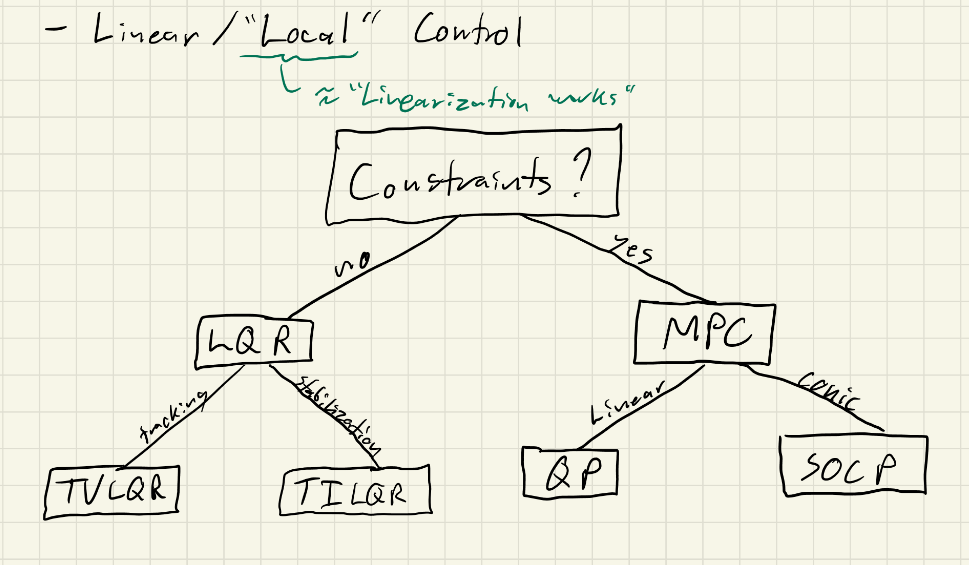
\includegraphics[width=\linewidth]{lecture_14_1.png}
\end{figure}


\section*{Nonlinear Trajectory Optimization/Planning}

\begin{table}[h]
    \centering
    \renewcommand{\arraystretch}{1.5}
    \begin{tabular}{c|c}
        \textbf{DIRCOL} & \textbf{DDP} \\
        \hline
        \textcolor{red}{Only respects dynamics at convergence} & \textcolor{teal}{Always dynamically feasible} \\
        \textcolor{teal}{Can use infeasible guess} & \textcolor{red}{Can only guess controls} \\
        \textcolor{teal}{Can handle arbitrary constraints} & \textcolor{red}{Hard to handle constraints} \\
        \textcolor{red}{Tracking controller must be designed separately} & \textcolor{teal}{TVLQR tracking controller is free} \\
        \textcolor{red}{Typically not as fast} & \textcolor{teal}{Very fast (local) convergence} \\
        \textcolor{red}{Difficult to implement large-scale SQP solver} & \textcolor{teal}{Easy to implement on embedded systems} \\
        \textcolor{teal}{Numerically robust} & \textcolor{red}{Has issues with ill-conditioning} \\
    \end{tabular}
\end{table}

\begin{itemize}
    \item \textbf{DDP} is often a good choice for \textit{online/real-time} applications where speed is critical and constraint tolerance is not critical.
    \item \textbf{DIRCOL} is often a good choice for \textit{offline} trajectory design, especially over long horizons and/or with complex constraints.
\end{itemize}

\noindent\rule{\textwidth}{0.4pt} % Horizontal line
\section*{Attitude}

\begin{itemize}
    \item Many robotic systems undergo \textbf{large rotations} (quadrotors, airplanes, spacecraft, underwater vehicles, legged robots).
    \item Naïve angle-based parameterizations (Euler angles) have \textbf{singularities} that cause failures and/or require hacks. \textbf{Never use them}
    \item Rotation matrices and quaternions are \textbf{singularity-free}, but optimizing over them requires some extra tricks. Both are over parameterized. using 9 numbers for rotation matrices and 4 numbers for quaternions, so have 6 and 1 constrains respectively because there are only 3 degrees of freedom.
    \item \textbf{What is Attitude?}
    rotation from some body frame on the robot to some fixed world frame. Left superscripts for frame being rotated to, right superscript for frame being rotated from
\end{itemize}
\begin{figure}[H]
    \centering
    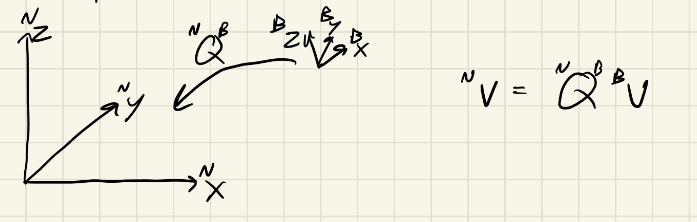
\includegraphics[width=\linewidth]{lecture_14_2.png}
\end{figure}
\begin{itemize}
    \item Rotation from body frame to world frame
    \item 3DOF, but there is no globally nonsingular 3-parameter attitude representation. 
\end{itemize}

\section*{Rotation / ``Direction-Cosine'' Matrix}

\[
\begin{bmatrix}
    ^N X_1 \\
    ^N X_2 \\
    ^N X_3
\end{bmatrix}
=
\underbrace{
\begin{bmatrix}
   & ^Bn_1^T& \\
    &^Bn_2^T &\\
   & ^Bn_3^T&
\end{bmatrix}
}_{^NQ^B}
\begin{bmatrix}
    ^B X_1 \\
    ^B X_2 \\
    ^B X_3
\end{bmatrix}
\]

\[
=
\begin{bmatrix}
\\
    ^Nb_1 &
    ^Nb_2 &
    ^Nb_3 \\
    \\
\end{bmatrix}
\begin{bmatrix}
    ^B X_1 \\
    ^B X_2 \\
    ^B X_3
\end{bmatrix}
\]
\begin{align*}
    \Rightarrow Q^TQ &= I \quad \Rightarrow Q^{-1} = Q^T
    \\
    & \hspace{1mm} \Rightarrow \text{``Orthogonal"}
    \\
    \Rightarrow det(Q) &= 1 \quad \text{``special"}
    \\
    &Q\in SO(3) \quad\text{``Special Orthogonal group in 3D"}
\end{align*}
Where a group is just a class of matrices with certain properties

\section*{Kinematics (How do I integrate a gyro?)}
\begin{figure}[H]
    \centering
    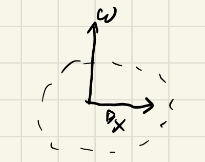
\includegraphics[width=0.25\linewidth]{lecture_14_3.png}
    \caption{A record spinning at some constant $\omega$}
\end{figure}

\begin{align*}
^N X &= Q(t)\ ^BX,
\quad
^N \dot{X} = \, ^N \omega \times \, ^N X
\\
&\hspace{32mm}= Q (\, ^B \omega \times \, ^B X)
\end{align*}

\textbf{Apply chain rule:}

\begin{align*}
^N X = Q \, ^B X \quad \Rightarrow \quad ^N \dot{X} = \dot{Q} \, ^B X + Q \, ^B \dot{X}
\\
^B X &= 0
\\
^N \dot{X} = \dot{Q} \, ^B X
\end{align*}

\[
\Rightarrow \quad \dot{Q} \, ^B X = Q (\, ^B \omega \times \, ^B X)
\]

\[
\omega \times x =
\begin{bmatrix}
    0 & -\omega_3 & \omega_2 \\
    \omega_3 & 0 & -\omega_1 \\
    -\omega_2 & \omega_1 & 0
\end{bmatrix}
\begin{bmatrix}
    x_1 \\ x_2 \\ x_3
\end{bmatrix}
= \hat{\omega} x
\]

\[
\Rightarrow \quad \dot{Q} \, ^B X = Q \hat{\omega} \, ^B X
\]

\[
\Rightarrow \quad \boxed{\dot{Q} =\ ^NQ^B \ ^B{\hat{\omega}}}
\]


\begin{itemize}
    \item We could do dynamics with rotation matrices in our state, but this has a lot of redundancy.
    \item Quaternions are more compact/efficient.
\end{itemize}

\section*{Quaternions}
\begin{itemize}
    \item Define axis of rotation (unit vector) $\mathbf{a}$.
    \item Define angle of rotation (scalar, radians) $\theta$.
\end{itemize}

\[
\boldsymbol{\phi} = \mathbf{a} \theta
\]
3D vector whos direction is $\theta$ and magnitude is $\mathbf{a}$
\[
\|\boldsymbol{\phi}\| = \theta, \quad \frac{\boldsymbol{\phi}}{\|\boldsymbol{\phi}\|} = \mathbf{a}
\]

\begin{itemize}
    \item For constant $\omega$ (for short $h$), we can think of $\boldsymbol{\phi}$ as the integral of $\omega$:
\end{itemize}

\[
\boldsymbol{\phi} \approx \int_0^h \omega(t) \, dt
\]

\[
\text{(not true in general)}
\]


\begin{itemize}
    \item In terms of $\boldsymbol{\phi}$, we can define quaternions:
\end{itemize}

\[
q =
\begin{bmatrix}
    \cos{(\Theta/2)} \\
    \mathbf{a} \sin{(\Theta/2)}
\end{bmatrix}
\leftarrow \begin{bmatrix}
    \text{``scalar part"} \\
    \text{``vector part"}
\end{bmatrix}
\]

\begin{itemize}
    \item $q^T q = 1 \quad \Rightarrow \quad$ Valid rotations correspond to ``unit quaternions''. Easy to normalize.
    \item $q$ and $-q$ correspond to the same rotation (adding $2\pi$ to $\Theta$). Called a ``double cover''.
    \item Operations on quaternions are analogous to rotation matrices.
\end{itemize}

\section*{Quaternion Multiplication}

\[
q_1 * q_2 =
\begin{bmatrix}
    s_1 \\ V_1
\end{bmatrix}
*
\begin{bmatrix}
    s_2 \\ V_2
\end{bmatrix}
=
\begin{bmatrix}
    s_1 s_2 - V_1^T V_2 \\
    s_1 V_2 + s_2 V_1 + V_1 \times V_2
\end{bmatrix}
\]

\[
=
\underbrace{
\begin{bmatrix}
    s_1 &- \hat{V}_1\\
    v_1 & s_1I+\hat{V}_1
\end{bmatrix}}_{L(q_1)}
\begin{bmatrix}
    s_2 \\ V_2
\end{bmatrix}
=
\underbrace{
\begin{bmatrix}
    s_2 & - \hat{V}_2^T \\
    V_2 & sI - \hat{V}_2
\end{bmatrix}
}_{R(q_2)}
\begin{bmatrix}
    s_2 \\ V_2
\end{bmatrix}
\]

\[
=
\underbrace{
\begin{bmatrix}
    s_2 I_{3\times3} - \hat{V}_2
\end{bmatrix}
}_{R(q_2)}
\begin{bmatrix}
    s_1 \\ V_1
\end{bmatrix}
\]

\section*{Quaternion Conjugate}

\[
q^\dagger =
\begin{bmatrix}
    s \\
    -V
\end{bmatrix}
=
T q =
\begin{bmatrix}
    1 & 0 \\
    0 & -I
\end{bmatrix}
\begin{bmatrix}
    s \\
    V
\end{bmatrix}
\]

\section*{Rotate a Vector}

\[
\begin{bmatrix}
    0 \\ X
\end{bmatrix}
=
q *
\begin{bmatrix}
    0 \\ ^B X
\end{bmatrix}
* q^\dagger
\]

\[
=
H^T L(q) R(q) H \ ^B X
\]

\[
H^T R^T(q) L(q) H\ ^B X
\]

\[
\text{(gives } Q(q) \text{)}
\]

\[
H X =
\begin{bmatrix}
    0 \\ X
\end{bmatrix}
\Rightarrow
H =
\begin{bmatrix}
    0 \\ I
\end{bmatrix}
\]
\section*{Quaternion Kinematics}

\[
\dot{q} = \frac{1}{2} q * 
\begin{bmatrix}
    0 \\ \omega
\end{bmatrix}
= \frac{1}{2} L(q) H \omega
\]

\[
\underbrace{L(q) H}_{4 \times 3}
\]

\begin{itemize}
    \item Now we can simulate dynamics with rotations.
\end{itemize}

\end{document}
